\documentclass[12pt,a4paper]{article}
\usepackage{geometry}
\usepackage{slashbox}
\geometry{
	a4paper,
	total={170mm,257mm},
	left=20mm,
	right=20mm,
	top=20mm,
	bottom=20mm
}
\usepackage{graphicx}
\usepackage{pdfpages}
\usepackage{placeins}
\usepackage{float}

\usepackage{polski}
\usepackage[utf8]{inputenc}

\begin{document}
	
	\begin{titlepage}
		\newgeometry{top=5.5cm, bottom=3cm}
		
		\centering
		{\huge\bfseries Logika układów cyfrowych lab.\par}
		
		\vspace{0.5cm}
		Prowadzący: Mgr inż. Antoni Sterna (E02-38m, wtorek 17:05) \\
	
		\vspace{1.1cm}
		{\Large sprawozdanie 4 - 2017.11.07\par}
		\vfill
		
		{\large\bfseries Jakub Dorda 235013\par}
		{\large\bfseries Marcin Kotas 235098\par}
		
		\vspace{1cm}
		\today \\ \LaTeX
		
		\restoregeometry
	\end{titlepage}

	
	\section{Wprowadzenie/cel ćwiczeń}
	
	
		
	\section{Licznik synchroniczny 3 bitowy rewersyjny}
		
		\subsection{Tabela prawdy i tablice Karnaugh:}
			
			
			
		\subsection{Minimalizacje:}
		
		
		
		\subsection{Użyte wzory:}
		
			
	
		\subsection{Schemat układu:}
		
			\vspace{1.5cm}
			\begin{center}
				\makebox[\textwidth]{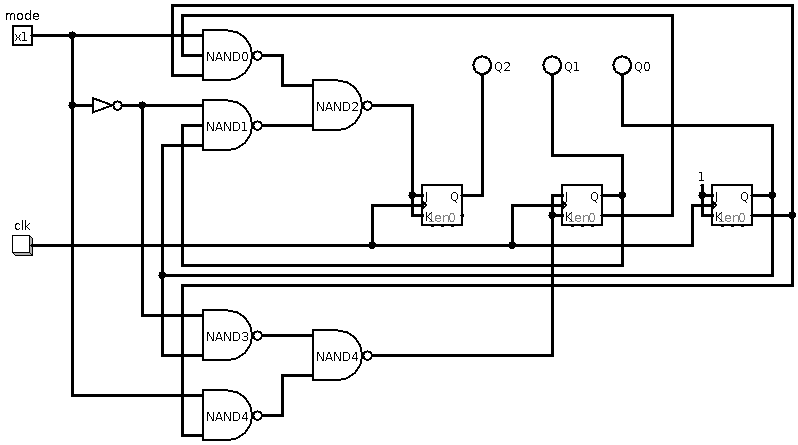
\includegraphics[width=\paperwidth - 30mm]{schem/circuit.png}}
				Schemat 1: 
			\end{center}
	
	\section{Licznik asynchroniczny modulo 4/11}
		
		\subsection{Tabela prawdy i tablice Karnaugh:}
			
			
	
		\subsection{Minimalizacje:}
			
		
			
		\subsection{Użyte wzory:}
		
			
			
		\subsection{Schemat układu:}
		
			\vspace{0.5cm}
			\begin{center}
				\makebox[\textwidth]{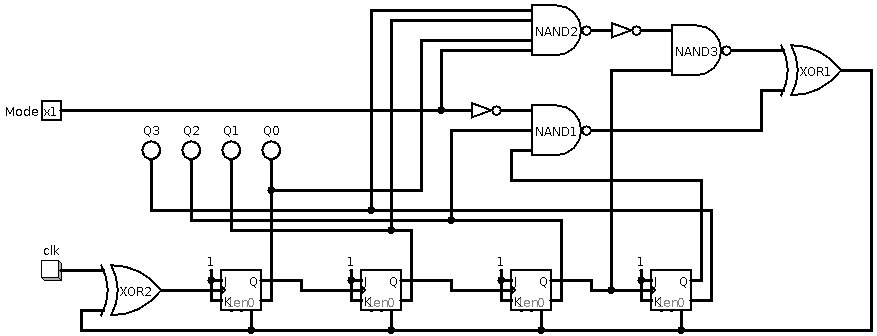
\includegraphics[width=\paperwidth - 20mm]{schem/circuit2.png}}
				Schemat 2: 
			\end{center}

	\section{Wnioski/podsumowanie}
	
	
\end{document}